
\newpage
\section{Analisi dei rischi} \label{AnalisiDeiRischi}
	Per svolgere un progetto in maniera \gloss{efficiente} ed \gloss{efficace}, viene effettuata un'analisi preliminare dei rischi che possono ostacolare il processo di sviluppo.
	È quindi fondamentale avere un sistema che ne permetta la gestione per poter reagire immediatamente e un piano di gestione ben definito in caso dovessero presentarsi.\\
	I seguenti punti rappresentano come è stato deciso di trattare i rischi:
	\begin{itemize}
		\item \textbf{Identificazione}: individuare i potenziali rischi che possono presentarsi
		\item \textbf{Analisi}: determinarne la probabilità di occorrenza e comprenderne la criticità
		\item \textbf{Pianificazione}: definire strategie che possono evitare i rischi precedentemente trovati
		\item \textbf{Controllo}: si monitorano e revisionano i rischi affinché non si realizzino nel corso del progetto
		\item \textbf{Revisione}: in caso dovessero presentarsi, dopo averli risolti, si rivede la strategia utilizzata e in caso ci siano migliorie possibili si rivede. Nel caso non fosse stata definita una strategia per tale rischio se ne definisce una.
	\end{itemize}
	\subsection{Valutazione}
	Per la valutazione dei rischi viene utilizzato uno strumento di misura chiamato \textit{Qualitative Risk Assessment}, che ne considera i criteri quantitativi e qualitativi assegnando a ciascuno un valore di gravità determinato dalla probabilità che il rischio possa avvenire e dalla gravità che esso pone al progetto.
	% VEDI : https://www2.deloitte.com/content/dam/Deloitte/it/Documents/risk/Board%20Academy%20Corso%20C6%2020%20dic%202012%20SDA%20Bocconi.pdf
	Dato il numero non elevato di rischi, si è scelto di mettere solamente tre livelli di gravità e probabilità producendo quindi una matrice con nove. In questo modo i rischi possono essere classificati in tre livelli di importanza:
	
	\begin{itemize}
		\item \textbf{Basso}
		\item \textbf{Medio}
		\item \textbf{Alto}
	\end{itemize}

	\begin{figure}[H]
		\centering
		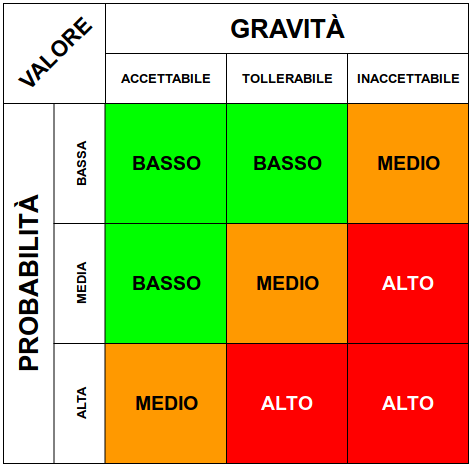
\includegraphics[scale=0.5]{img/risk_assessment_table.png}\\
		\caption{Matrice del Qualitative Risk Assessment}
	\end{figure}
	\subsection{Tipologia}
	Le tipologie in cui suddividere i rischi sono state prese dal libro Software Engineering\footnote{Software Engineering, 10° edizione, Pagina 648, Capitolo 22: Project management} e sono,:
	\begin{itemize}
 		\item \textbf{Organizzativo}: dovuto alla gestione di persone che hanno diverse responsabilità all'interno progetto
		\item \textbf{Personale}: riguarda le conoscenze, i tempi e la formazione personale
		\item \textbf{Requisiti}: ha a che fare con il numero di requisiti che può variare nel corso del tempo
		\item \textbf{Strumentale}: per la performance degli strumenti
		\item \textbf{Tecnologico}: per problemi riguardanti le tecnologici.
	\end{itemize}
	\subsection{Classificazione}
	A ciascun rischio viene assegnato un codice identificativo in modo da essere facilmente riconoscibile e per comprenderne le generalità (classe, probabilità e severità), per poi non doverle cercare nelle tabelle che comprendono tutti i rischi del progetto analizzati.
	
	Questo codice è composto da:
	
	\begin{center}
		\texttt{[Tipologia][ID]-[Gravità][Probabilità][Classe]}
	\end{center}

	I valori che possono assumere sono:
	
	\begin{itemize}
		\item \textbf{Tipologia}:
			\begin{itemize}
				\item \textbf{O}: organizzativo
				\item \textbf{P}: personale
				\item \textbf{R}: requisiti
				\item \textbf{S}: strumentale
				\item \textbf{T}: tecnologico.
			\end{itemize}
		
		\item \textbf{ID}: numero progressivo di tre cifre che inizia da uno (001 - 999)
		\item \textbf{Gravità}:
			\begin{itemize}
				\item \textbf{0}: accettabile
				\item \textbf{1}: tollerabile
				\item \textbf{2}: inaccettabile.
			\end{itemize}
		
		\item \textbf{Probabilità}:
			\begin{itemize}
				\item \textbf{0}: bassa
				\item \textbf{1}: media
				\item \textbf{2}: alta.
			\end{itemize}
		
		\item \textbf{Classe}:
			\begin{itemize}
				\item \textbf{0}: basso
				\item \textbf{1}: medio
				\item \textbf{2}: alto.
			\end{itemize}
	\end{itemize}

	Ad esempio con P01-021 si può intuitivamente capire, conoscendo la legenda, che si tratta di un rischio del personale, con un numero progressivo 01, di gravità accettabile, probabilità alta e un valore di classe medio.
	
	\subsection{Lista rischi possibili}
	Per elencare i rischi viene la seguente struttura tabellare:
	\begin{table}[H]
		\begin{risktable}{\columnwidth}{m{1.5cm}m{11.7cm}}
			\thead{ID} & 
			\thead{Nome significativo}\\
			\hline
			\rowcolor{gray!15}
			\multicolumn{2}{X}{
				\thead{Breve descrizione}
			}\\
			\hline
			\multicolumn{2}{X}{
				\thead{Strategie per la rilevazione}
			}\\
			\hline
			\rowcolor{gray!15}
			\multicolumn{2}{X}{
				\thead{Contromisure e mitigazione}
			}\\
		\end{risktable}
		\caption[Analisi dei rischi]{Struttura della tabella dell'analisi dei rischi}
	\end{table}

	\noindent
	Dopo un'attenta analisi del capitolato e alcuni incontri tra dei componenti del team di sviluppo, è stato deciso di catalogare i seguenti rischi elencati in maniera crescente rispetto all'ID:\\
	
	\mydoublerule{\linewidth}{0pt}{2pt}
	
	\begin{table}[H]
		\begin{risktable}{\columnwidth}{m{1.5cm}m{13.5cm}}
			\thead{P001-111} & 
			Inesperienza del team a livello tecnico\\
			\hline
			\rowcolor{gray!15}
			\multicolumn{2}{X}{
				\textbf{Descrizione}: non tutti i componenti del team di sviluppo hanno le conoscenze di ambienti di sviluppo, linguaggi di programmazione e strumenti richiesti dall'azienda allo stesso livello.
			}\\
			\hline
			\multicolumn{2}{X}{
				\textbf{Strategia}: sarà compito del \Res\ di progetto parlare con il resto del team di sviluppo e capire ciascuno che conoscenze ha delle tecnologie da utilizzare per sviluppare il progetto.
			}\\
			\hline
			\rowcolor{gray!15}
			\multicolumn{2}{X}{
				\textbf{Mitigazione}: ciascun componente si impegna a sanare le proprie lacune e portarsi ad un livello comune concordato in modo da poter lavorare autonomamente e potersi prendere impegni risolvibili senza dover usare tempo ulteriore per imparare la tecnologia.
			}\\
		\end{risktable}
	\end{table}

	\mydoublerule{\linewidth}{0pt}{2pt}

	\begin{table}[H]
		\begin{risktable}{\columnwidth}{m{1.5cm}m{13.5cm}}
			\thead{P002-122} & 
			Impreparazione del team a livello gestionale \\
			\hline
			\rowcolor{gray!15}
			\multicolumn{2}{X}{
				\textbf{Descrizione}: non avendo affrontato progetti del genere prima d'ora, i componenti del team di sviluppo non conoscono bene i ruoli che devono intraprendere e i compiti da svolgere.				
			}\\
			\hline
			\multicolumn{2}{X}{
				\textbf{Strategia}: sarà compito del componente che fa da \Res\ assicurarsi che non ci siano perplessità da parte degli altri membri sui ruoli ricoperti e sui compiti assegnati.
			}\\
			\hline
			\rowcolor{gray!15}
			\multicolumn{2}{X}{
				\textbf{Mitigazione}: durante le ore di studio personale, ciascun componente si impegna a studiare la gerarchia dei ruoli\protect\footnotemark e in caso di dubbi ne potrà parlare con il team di sviluppo oppure direttamente con chi fa da \Res\.
			}\\
		\end{risktable}
	\end{table}

	\footnotetext{Nei Riferimenti informativi - Vincoli di organigramma e specifiche economiche}
	
	\mydoublerule{\linewidth}{0pt}{2pt}
		
	\begin{table}[H]
		\begin{risktable}{\columnwidth}{m{1.5cm}m{13.5cm}}
			\thead{P003-100} & 
			Approvazione errata di documenti \\
			\hline
			\rowcolor{gray!15}
			\multicolumn{2}{X}{
				\textbf{Descrizione}: è possibile che il \Res\ commetta errori nella fase di approvazione dei documenti che possono portare alla consegna di documentazione errata o scadente, causando quindi disguidi con il cliente, oltre che a lasciare un'impressione negativa. \'E necessario correggere tali sviste, andando quindi a sprecare risorse investibili in altri compiti.
			}\\
			\hline
			\multicolumn{2}{X}{
				\textbf{Strategia}: colui che svolge il ruolo di \Res\ deve avere modo di controllare il lavoro prodotto dal proprio team in modo costante e graduale.
			}\\
			\hline
			\rowcolor{gray!15}
			\multicolumn{2}{X}{
				\textbf{Mitigazione}: chi svolge il ruolo di \Res\ deve assicurarsi che i documenti approvati siano effettivamente validi e in caso di sviste il \Ver\ deve saper trovare e correggere gli eventuali errori.
			}\\
		\end{risktable}
	\end{table}
	
	\mydoublerule{\linewidth}{0pt}{2pt}
	
	\begin{table}[H]
		
		\begin{risktable}{\columnwidth}{m{1.5cm}m{13.5cm}}
			\thead{P004-100} & 
			Cattiva gestione dell'archivio per la documentazione del progetto\\
			\hline
			\rowcolor{gray!15}			
			\multicolumn{2}{X}{
				\textbf{Descrizione}: data la poca esperienza dei componenti del team di sviluppo con progetti di questo calibro, dove la documentazione è una delle parti principali, gestirla può risultare una novità e potrebbe presentare difficoltà nella gestione.
			}\\
			\hline
			\multicolumn{2}{X}{
				\textbf{Strategia}: l'\Amm\ deve aver predisposto una repository comune in cui ciascun componente potrà caricare il proprio lavoro e dovrà saperla utilizzare in maniera tale da non andare a modificare quel che è stato caricato dagli altri.
			}\\
			\hline
			\rowcolor{gray!15}			
			\multicolumn{2}{X}{
				\textbf{Mitigazione}: in caso di errori nella gestione della repository, l'\Amm\ deve saperli risolvere in maniera tempestiva in modo da evitare che chi andrà ad utilizzare successivamente la repository scarichi file errati propagando l'errore anche sul proprio sistema.
			}\\
		\end{risktable}
		
	\end{table}

	\mydoublerule{\linewidth}{0pt}{2pt}
	
	\begin{table}[H]
		\begin{risktable}{\columnwidth}{m{1.5cm}m{13.5cm}}			
			\thead{P005-021} & 
			Intesa parziale tra i membri del team di sviluppo\\
			\hline
			\rowcolor{gray!15}
			\multicolumn{2}{X}{
				\textbf{Descrizione}: il team di sviluppo è formato principalmente da persone che precedentemente non si conoscevano o che hanno avuto poche interazioni tra di loro fino al momento della creazione di quest'ultimo. Poiché non si conoscono le competenze altrui, ciò può comportare un'errata gestione del lavoro e assegnazione dei compiti.
			}\\
			\hline
			\multicolumn{2}{X}{
				\textbf{Strategia}: attraverso gli incontri diretti o con strumenti di chat quali Telegram o Slack, ci si confronta e si realizzano i diversi modi di lavorare per ognuno.
			}\\
			\hline
			\rowcolor{gray!15}
			\multicolumn{2}{X}{
				\textbf{Mitigazione}: il team di sviluppo si impegna a conoscersi nel corso delle riunioni e ritrovi. Si discute inoltre insieme di un way of working comune che possa soddisfare le metodologie di lavoro di tutti i componenti.
				Nel caso in cui nascano dibattiti o sia difficile raggiungere un punto d'intesa, la decisione è presa dalla maggioranza.
				%e democrazia sia... purtroppo
				%In caso ci fossero dibattiti, per non ricorrere alle lame, gli altri componenti andranno a calmare le acque senza che ci siano morti.
				%LOOOL
			}\\
		\end{risktable}
		
	\end{table}
				
	\mydoublerule{\linewidth}{0pt}{2pt}
		
	\begin{table}[H]
		
		\begin{risktable}{\columnwidth}{m{1.5cm}m{13.5cm}}
			\thead{P006-122} & 
			Cattiva amministrazione delle risorse \\
			\hline
			\rowcolor{gray!15}
			\multicolumn{2}{X}{
				\textbf{Descrizione}: data l'inesperienza del team di sviluppo con progetti di questa natura è possibile che sorgano errori nell'amministrazione delle risorse come tempo, costi e suddivisione dei ruoli.
			}\\
			\hline
			\multicolumn{2}{X}{
				\textbf{Strategia}: a ciascuna riunione di \gruppo\ si controllerà se il lavoro svolto finora è pertinente a quanto è stato preventivato, modificando di conseguenza il consuntivo e il preventivo a finire.
				Tramite strumenti come diagrammi di \gloss{Gantt} dinamici, dove ciascun componente può aggiornare i tempi previsti per completare l'attività assegnata, è possibile monitorare costantemente il progresso del progetto in modo tale da evitare situazioni di \gloss{zero laxity}.
			}\\
			\hline
			\rowcolor{gray!15}			
			\multicolumn{2}{X}{
				\textbf{Mitigazione}: in caso dovessero sorgere problemi di questa natura, AlphaPix si impegnerà a ridistribuire le risorse in modo da rispettare la tabella di marcia e in particol modo le scadenze, tenendo conto di consegnare comunque un prodotto di qualità.
			}\\
		\end{risktable}
		
	\end{table} 

	\mydoublerule{\linewidth}{0pt}{2pt}
	
	\begin{table}[H]
		\begin{risktable}{\columnwidth}{m{1.5cm}m{13.5cm}}		
			\thead{O001-201} & 
			Ritardo consegna del materiale per una revisione oltre la scadenza \\
			\hline
			\rowcolor{gray!15}
			\multicolumn{2}{X}{
				\textbf{Descrizione}: è possibile che uno o più componenti del team di sviluppo, per impegni legati alla propria vita privata e universitaria, non riescano a gestire i compiti assegnati e quindi arrivare ad una scadenza senza aver finito il proprio lavoro, obbligando l'intero team di sviluppo rinviare la consegna.
			}\\
			\hline
			\multicolumn{2}{X}{
				\textbf{Strategia}: sarà compito del \Res\ assicurarsi che il lavoro proceda in maniera lineare ponendo scadenze intermedie, monitorando il lavoro del team di sviluppo, organizzando riunioni e aggiornandosi sullo stato dei vari compiti assegnati secondo il way of working scelto.
			}\\
			\hline
			\rowcolor{gray!15}			
			\multicolumn{2}{X}{
				\textbf{Mitigazione}: ciascun membro si impegna a gestire il proprio tempo adeguatamente in rapporto con gli altri impegni universitari senza tralasciare il suo ruolo nel team di sviluppo: distinguendo le priorità in modo da non influenzare negativamente lo sviluppo del progetto. In caso di impegni che possano ostacolare ciò, ci si prenderà cura di avvisare gli altri componenti del team di sviluppo per tempo.
			}\\
		\end{risktable}
	\end{table}
	
	\mydoublerule{\linewidth}{0pt}{2pt}
	
	\begin{table}[H]
		\begin{risktable}{\columnwidth}{m{1.5cm}m{13.5cm}}
			\thead{O002-010} & 
			Mancanza di comunicazione con l'azienda \\
			\hline
			\rowcolor{gray!15}
			\multicolumn{2}{X}{
				\textbf{Descrizione}: durante lo sviluppo del progetto è possibile che AlpaSix non contatti i rappresentanti dell'azienda e che questi quindi non siano al corrente dei progressi fatti, dei requisiti completati e del modo in cui si ha lavorato.
			}\\
			\hline
			\multicolumn{2}{X}{
				\textbf{Strategia}: è opportuno che il \Res\ si metta in comunicazione con l'azienda, attraverso Telegram, Skype o tramite incontri di persona, e riferisca il progresso svolto dal team di sviluppo in modo da avere feedback e critiche costruttive che possano migliorare lo sviluppo del progetto.
			}\\
			\hline
			\rowcolor{gray!15}			
			\multicolumn{2}{X}{
				\textbf{Mitigazione}: in caso di mancata comunicazione per un lungo arco di tempo è opportuno che alla prima scadenza di revisione utile il team di sviluppo si impegni a contattare l'azienda per avere un suo feedback.
			}\\
		\end{risktable}
		
	\end{table} 	
	
	\mydoublerule{\linewidth}{0pt}{2pt}
		
	\begin{table}[H]
		\begin{risktable}{\columnwidth}{m{1.5cm}m{13.5cm}}
			\thead{S001-100} & 
			Problematiche hardware \\
			\hline
			\rowcolor{gray!15}			
			\multicolumn{2}{X}{
				\textbf{Descrizione}: è possibile che i computer e altri strumenti hardware che possono essere utilizzati dai membri del team di sviluppo risultino difettosi o smettano di funzionare.
			}\\
			\hline
			\multicolumn{2}{X}{
				\textbf{Strategia}: ciascun membro avrà cura degli strumenti a sua disposizione in modo tale che non sorgano problemi che possano ostacolare il lavoro.
			}\\
			\hline
			\rowcolor{gray!15}			
			\multicolumn{2}{X}{
				\textbf{Mitigazione}: i guasti di natura hardware non sono facilmente prevedibili e in caso dovessero presentarsi è possibile utilizzare temporaneamente i computer forniti dai laboratori dell'università fino a quando la macchina difettosa non venga riparata o, se necessario, sostituita.
			}\\
		\end{risktable}
	\end{table}	
	
	\mydoublerule{\linewidth}{0pt}{2pt}
	
	\begin{table}[H]
		
		\begin{risktable}{\columnwidth}{m{1.5cm}m{13.5cm}}
			\thead{R001-122} & 
			Interpretazione errata dei requisiti: aggiunta o modifica di requisiti in corso di sviluppo \\
			\hline
			\rowcolor{gray!15}
			\multicolumn{2}{X}{
				\textbf{Descrizione}: durante il progetto, dopo aver effettuato una prima analisi di tutti i requisiti, può nascere il bisogno di modificare un requisito già fissato o aggiungerne uno non identificato in precedenza.
			}\\
			\hline
			\multicolumn{2}{X}{
				\textbf{Strategia}: è possibile che nel corso dello sviluppo del progetto vengano scoperti requisiti secondari impliciti non precedentemente valutati che necessitano di essere sviluppati.
				A ciascuna milestone, anche intermedia, è utile controllare che la lista dei requisiti da svolgere sia coerente con quella richiesta dall'azienda analizzando il documento che presenta il loro capitolato.
			}\\
			\hline
			\rowcolor{gray!15}			
			\multicolumn{2}{X}{
				\textbf{Mitigazione}: nel caso dovesse sorgere la necessità di sviluppare requisiti inaspettati, questi andranno analizzati per capire di che risorse hanno bisogno e come andranno inseriti nella scaletta di sviluppo del progetto in modo adeguato. Data la natura modulare del progetto, ciascun requisito verrà sviluppato dal più al meno importante in modo da dover svolgere compiti facilmente monitorabili e testabili.
			}\\
		\end{risktable}
		
	\end{table}
	
	\mydoublerule{\linewidth}{0pt}{2pt}
	
	\begin{table}[H]
		
		\begin{risktable}{\columnwidth}{m{1.5cm}m{13.5cm}}
			\thead{T001-100} & 
			Problematiche software\\
			\hline
			\rowcolor{gray!15}
			\multicolumn{2}{X}{
				\textbf{Descrizione}: il team di sviluppo fa affidamento a prodotti software per l'integrazione del codice e dei documenti. Eventuali problemi possono causare gravi perdite di dati.
			}\\
			\hline
			\multicolumn{2}{X}{
				\textbf{Strategia}: siccome ci si affida a servizi di terze parti, i malfunzionamenti che possono capitare sono imprevedibili, ma data la nota affidabilità di questi strumenti la probabilità che questo rischio accada è molto bassa.
			}\\
			\hline
			\rowcolor{gray!15}
			\multicolumn{2}{X}{
				\textbf{Mitigazione}: ciascun componente si impegna a mantenere una copia, aggiornata periodicamente, della repository contenente il proprio lavoro, nella propria macchina o eventualmente in una memoria esterna.
			}\\
		\end{risktable}
		
	\end{table}
	
	\mydoublerule{\linewidth}{0pt}{2pt}